\documentclass[smallextended]{svjour3}

\usepackage{graphicx}
\usepackage{amsmath,amssymb}
\usepackage{booktabs}
\usepackage{tabularx}
\usepackage{multirow}
\usepackage{url}
\usepackage{xurl}
\usepackage{natbib}
\usepackage{seqsplit}

\providecommand{\doi}[1]{\url{https://doi.org/#1}}
\providecommand{\urlprefix}{URL }

\journalname{Journal of Geodesy}

\begin{document}

\title{A reproducible benchmark of deep learning versus classical signal
decomposition for GNSS coordinate time series: denoising, gap filling, offset
detection, and their impact on station velocity and coloured noise}

\author{Qinghua Zhang \and Zhengsheng Chen}

\institute{Qinghua Zhang \at School of Geography, Nanjing Normal University,
Nanjing 210023, China \email{sqmha@126.com} (ORCID 0000-0003-3578-3749) \and
Zhengsheng Chen \at PLA Rocket Force University of Engineering, Xi'an 710025,
China \email{czsgeo@126.com} (ORCID 0000-0003-0628-3470)}

\authorrunning{Q. Zhang and Z. Chen}
\titlerunning{A reproducible benchmark of learned and classical GNSS processing}

\date{Received: date / Accepted: date}

\maketitle

\begin{abstract}
A GNSS station velocity is only as defensible as the coloured-noise model behind
its uncertainty, yet deep learning is now proposed for every step of the
coordinate-series pipeline and is usually judged by signal-recovery error alone.
We build a reproducible benchmark on 333 daily coordinate series from 321 sites,
with a station-level split, frozen station lists, fixed seeds and injected
white-plus-flicker noise, and we score classical and learned methods on
denoising, gap filling and offset detection and then on the published product,
the secular velocity and its uncertainty. The protocol removes three confounds of
an earlier version: the ground truth is drawn from both an in-family and an
out-of-family signal, the network is evaluated under the normalisation used in
training, and detection is scored against real catalogue labels as well as
injected offsets. The verdict is task-specific. The parametric trajectory model
removes $0.790$ of the injected denoising error when the truth lies in its basis
but adds error ($-0.106$) when it does not; the learned denoiser is nearly
family-invariant ($0.366$ and $0.363$) and, with per-window inference, beats
every model-free decomposition in both truth families, though not the
parametric estimator when the truth lies in its basis. With per-window inference the learned gap filler is
the best method at 30-day synthetic gaps ($3.07$~mm), but on the full held-out
real set it ties linear interpolation on NGL ($2.964$ against $2.967$~mm) and
falls $0.06$~mm behind it on JPL, while the trajectory model remains best at
120 days. The learned
detector has higher average precision at 16--25~mm offsets but a lower
validation-selected $F_1$ at every amplitude, and on 1\,743 real catalogue labels
it averages $0.232$ (U-Net) and $0.273$ (TCN) against $0.457$ for the classical
detector, with four of thirty seeds collapsing. Downstream, no method improves the velocity: with protocol-matched
inference the learned denoiser reaches $0.0605$~mm\,yr$^{-1}$ and the learned
imputer $0.0586$, against $0.0586$--$0.0616$ for the untreated series and the
classical denoisers, and calibration stays near $0.65$ for all of them. The
factor-of-$3.6$ degradation and calibration collapse reported in the earlier
version were produced by whole-series normalisation. Adding a random-walk
component lowers absolute accuracy for every method without changing the
ordering. Learned gap filling at intermediate gaps is competitive on synthetic
records and no better than interpolation on the full real set; learned
denoising upstream of a velocity and noise fit is neither an improvement nor a
penalty.

\end{abstract}

\keywords{GNSS coordinate time series \and coloured noise \and power-law noise
\and denoising \and gap filling \and offset detection \and deep learning \and
benchmarks}

\section{Introduction}
\label{sec:intro}

A GNSS station velocity is a small number extracted from a long, noisy, interrupted
record. Its value is used in terrestrial reference frames \citep{altamimi2017pmm},
strain-rate fields \citep{kreemer2014gsrm} and loading studies
\citep{blewitt2002annual}, but its uncertainty is set less by the number of daily
solutions than by the time-correlated part of the coordinate error. A velocity
computed under a white-noise assumption can be optimistic by an order of
magnitude; the power-law noise model and the maximum-likelihood trajectory fit
that account for it are therefore not refinements but the basis of a defensible
velocity \citep{mao1999noise,williams2003coloured,amirisimkooei2007noise}.

Deep learning is now proposed for nearly every step before that fit: denoising,
gap filling and offset detection. Reported gains are large but rarely comparable,
because each study uses its own stations, its own metric and its own baseline.
The evaluation usually stops at signal recovery. A geodesist does not publish a
denoised series; they publish a velocity and an uncertainty, and a method can
improve recovery error while corrupting the noise estimate from which the
uncertainty is built.

This paper is a benchmark, not a new architecture. It asks a narrow question:
under one frozen protocol, on held-out real stations, does any learned method
beat a well-implemented classical one on the three tasks and on the products that
follow them? The answer is conditional rather than uniform. The parametric
baseline keeps its denoising advantage only while the truth stays inside its
basis; the learned gap filler wins at 30-day synthetic gaps once inference
matches training but does not beat linear interpolation on the full held-out
real set, and loses at long gaps; the learned detector orders large offsets
better but operates worse, and on real catalogue labels it trails in both $F_1$
and seed stability. The downstream product narrows the picture rather than
sharpening it: learned denoising reduces signal error, yet under the corrected
inference it neither improves nor degrades the velocity and its uncertainty.
The evidence behind this picture is stronger than in our first version in four
ways that matter.

First, the ground truth is no longer confined to the family the parametric
baseline assumes. In the earlier protocol the injected signal was a trend plus
constant harmonics, so the maximum-likelihood trajectory model was scored on its
own model family and removed about four-fifths of the injected error. We now
score the same methods on two truth families: an in-family signal built from a
real station's robust trajectory fit, and an out-of-family signal that adds
non-stationary seasonal amplitude, exponential transients and logarithmic
post-seismic relaxation. The parametric estimator loses its advantage when the
truth leaves its basis. The learned denoiser is nearly invariant across the two
families and, under protocol-matched inference, beats every model-free
decomposition in both; it remains far below the parametric estimator when the
truth sits in its basis.

Second, offset detection is evaluated against real catalogued offsets rather
than only against injected ones. We match the NGL discontinuity catalogue to the
held-out stations, keep labels inside each record and above the local noise
level, and score the classical detector and the learned detectors on the same
epochs. This removes the objection that synthetic offsets are easier than real
ones and tests the detectors where a geodesist would use them.

Third, training-seed variation is treated as part of the result. Denoising and
gap filling use ten seeds per architecture; detection uses twenty U-Net seeds
and ten TCN seeds. We report the
distribution over seeds, not a favourable draw, and we separate a fixed
read-out threshold from a threshold selected on held-out validation data. A
second architecture, a temporal convolutional network, is trained under the same
budget so that the conclusion is not a statement about one network.

Fourth, the downstream analysis includes a random-walk component. The first
version injected white plus flicker noise and left random walk open; here the
same velocity pipeline is run with and without a random-walk term, and the
effect on velocity bias, reported uncertainty and interval coverage is measured
rather than assumed. The benchmark also carries a second analysis centre: the
NGL long records are the primary set, and the held-out JPL series form an
external validation arm. JPL series from training sites contribute to training,
but no held-out site, from either centre, is ever seen by a learned method
before scoring.

The contributions are:

\begin{enumerate}
\item A reproducible benchmark of 333 daily series from 321 sites, with a
station-level 60/20/20 split (198/68/67 series, 193/64/64 sites), frozen station
lists, fixed seeds and released result files (Sec.~\ref{sec:data}).
\item A two-family ground-truth protocol that separates in-family from
out-of-family truth and shows how much of the classical advantage in the
earlier benchmark came from the truth sitting inside the parametric basis
(Sec.~\ref{sec:results:t1}).
\item A real-label offset study on 153 held-out component series from 58
stations, using 1\,743 catalogued discontinuities, with amplitude- and
signal-to-noise-stratified scores and detection delays
(Sec.~\ref{sec:results:t3:real}).
\item Seed- and architecture-robust comparisons for denoising, gap filling and
detection, including parameter counts, training cost and validation-based
threshold selection (Secs.~\ref{sec:results:t1}--\ref{sec:results:t3}).
\item A downstream propagation study under white-plus-flicker and
white-plus-flicker-plus-random-walk noise, reporting velocity bias, uncertainty
calibration and coverage, plus an external JPL arm and a regional holdout
(Secs.~\ref{sec:results:downstream} and~\ref{sec:results:external}).
\end{enumerate}

Section~\ref{sec:related} positions the benchmark against the four literatures it
joins. Section~\ref{sec:data} describes the data and the split,
Sec.~\ref{sec:method} the protocol and methods, and Sec.~\ref{sec:results} the
results. Section~\ref{sec:discussion} states the boundary of the conclusion and
its limitations, and Sec.~\ref{sec:conclusion} answers the question posed above.

\begin{figure}[t]
\centering
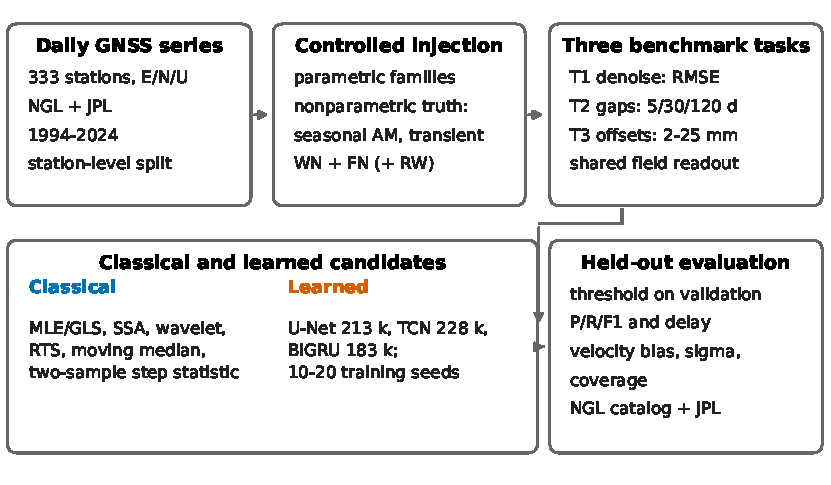
\includegraphics[width=\linewidth]{figures/fig01_pipeline.pdf}
\caption{The benchmark pipeline. Real daily series are injected with a known
signal and noise model, the resulting realisation is scored on the three tasks
by classical and learned candidates under one read-out rule, and each output is
carried into the velocity and noise estimation. The downstream step is what
separates a processing benchmark from a signal-recovery benchmark.}
\label{fig:pipeline}
\end{figure}


\section{Related work}
\label{sec:related}

Four literatures meet in this benchmark: coloured-noise modelling, model-free
decomposition, machine learning on coordinate series, and shared evaluation
protocols. Table~\ref{tab:related} summarises what each provides and what it
leaves out; the text keeps only the points that shape the protocol.

\paragraph{Coloured noise and the trajectory model.}
Power-law noise in daily coordinates and its control on velocity precision are
the founding results of the field \citep{mao1999noise,williams2003coloured}.
The maximum-likelihood trajectory fit, with efficient covariance construction and
support for missing epochs, is implemented in CATS \citep{williams2008cats} and
Hector \citep{bos2008fast,bos2013fast}, and the noise model has been extended to
multivariate and seasonal formulations
\citep{amirisimkooei2007noise,amirisimkooei2009multivariate,klos2018seasonal},
including stochastic seasonality in velocity estimation
\citep{xu2025velocity}.
This literature supplies our reference estimator and the generalised-least-squares
velocity covariance. It treats the trajectory model as the frame within which
everything is measured; we instead score it as one candidate among several,
including on gap filling and detection, which its formulation was not designed
for.

\paragraph{Model-free decomposition.}
Singular spectrum analysis \citep{wdowinski1997spatial,ji2024ssa}, wavelet
shrinkage \citep{ji2020wavelet}, multivariate SSA
\citep{gruszczynska2017mssa} and spatiotemporal PCA/Karhunen--Lo\`eve filtering
\citep{dong2006spatiotemporal} separate seasonal signal from residual without a
parametric trajectory. They are
the natural classical competitors for a learned model, and we carry SSA, wavelet
shrinkage and a moving median as three independent members of this family. Their
usual validation is the task they were built for, on the series they were built
on; here they are scored on the same injected realisations as every other method.

\paragraph{Learned processing.}
Networks have been applied to discontinuity detection
\citep{crocetti2021discontinuity,wang2025changepointcnn}, denoising
\citep{li2018denoising,mastella2025denoising,gao2022gbdt,he2026tspredictor},
gap filling as low-rank completion \citep{liu2022imputation}, network-wide
denoising with graph models \citep{bachelot2025gnn}, and uncertainty propagation
\citep{kiani2022uncertainty}, and decomposition-plus-learning pipelines have been
evaluated for height-series prediction \citep{guo2026decomposition}. Time-domain
machine learning for GNSS series has also been reviewed as a whole
\citep{gabsatarov2025review}; related variants continue to appear
\citep{simsek2025dl,ozarpaci2024machine}. The evidence is usually recovery error
on the task the network was trained for. Where a geodetic product is reached, the
velocity is often estimated directly from positions rather than through the
coloured-noise model, so the effect of processing on the published uncertainty is
not traced. That is the step this benchmark adds.

\paragraph{Shared protocols.}
DOGEx fixed a detection dataset, injected known offsets and had independent
groups run detectors blind \citep{gazeaux2013detecting}; it remains the model for
a community protocol, but it covers one task and synthetic truth. CATS and Hector
are tools, not protocols. We are not aware of a protocol that fixes the data and
the split, creates exact truth by injection, scores classical and learned methods
on the same realisations across three tasks, validates detection against real
catalogue labels, and carries each output through to velocity, noise amplitudes
and interval coverage.

\begin{table*}[t]
\centering
\caption{Positioning of representative work. ``Downstream'' means the study
reports the effect of processing on a geodetic product (velocity or its
uncertainty); ``common truth'' means classical and learned methods are scored on
the same known realisation.}
\label{tab:related}
\footnotesize
\setlength{\tabcolsep}{3pt}
\begin{tabularx}{\textwidth}{@{}p{2.4cm}p{2.0cm}Xp{1.7cm}p{2.8cm}@{}}
\toprule
Study or family & Task & Evidence base & Downstream & What this benchmark adds \\
\midrule
MLE trajectory; CATS, Hector & noise, velocity & parametric fit to real series & yes & scores the same estimator against nonparametric truth and other methods \\
SSA, wavelet, mSSA & decomposition & recovery on selected series & no & common realisations, three tasks, seed-aware learned comparison \\
Detection networks & offset detection & synthetic or station-specific labels & no & real catalogue labels, amplitude and SNR strata, delay \\
Denoising, imputation, GNN networks & T1, T2 & recovery error & no & downstream noise and uncertainty, gap lengths to one year \\
Learned uncertainty and velocity & product & direct velocity from positions & partial & processing-to-noise-to-uncertainty chain \\
DOGEx & detection & blind synthetic injection & no & three tasks, real labels, two analysis centres \\
This paper & T1--T3 & injection, two truth families, real labels & yes & station-level split, 10--20 seeds, two architectures, RW arm \\
\bottomrule
\end{tabularx}
\end{table*}


\section{Data and processing}
\label{sec:data}

The benchmark uses daily GPS coordinate series from two analysis centres. The
NGL long records are the primary set because they carry the multi-decade
histories needed for velocity and noise estimation; the JPL single-analysis-centre
series provide an independent processing arm and, at the held-out sites, an
external validation set. We do not use the IGS combination, whose combination
step has already repaired offsets and outliers and would remove the features the
detection task is meant to find \citep{dow2009igs,rebischung2016igs}.

\paragraph{Sources.}
NGL \texttt{tenv3} daily coordinates in ITRF, in millimetres, contribute 298
series \citep{blewitt2018ngl}. The JPL daily solutions contribute 35 series. Twelve sites appear in both
sources and therefore contribute two series each, so the benchmark holds 333
series from 321 unique sites. Series are labelled by source and site, and every
method is scored per component; no method sees the site label at test time.
Fig.~\ref{fig:sample} shows one held-out station before and after injection.

\begin{figure}[t]
\centering
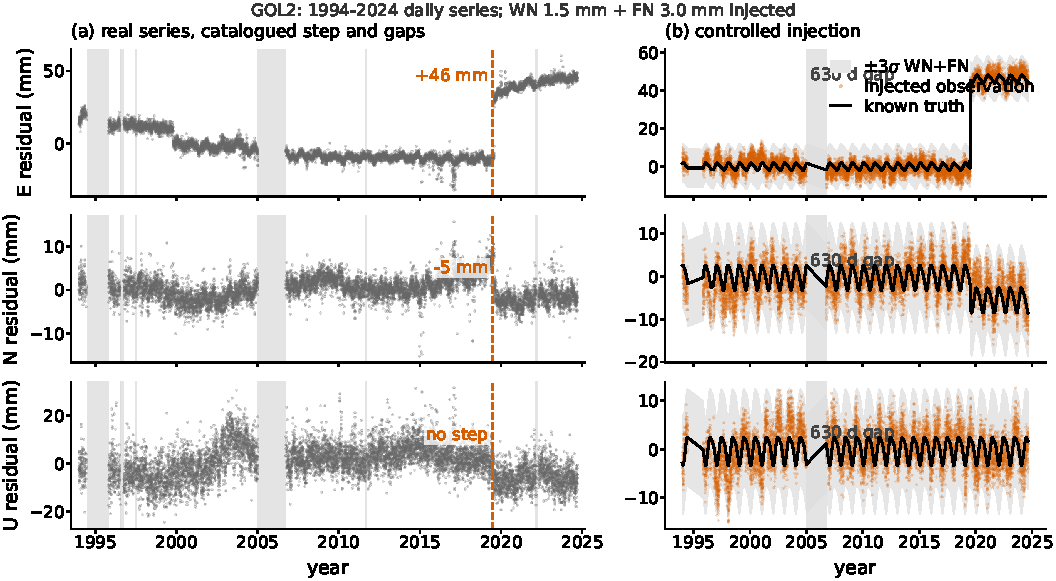
\includegraphics[width=\linewidth]{figures/fig02_real_sample.pdf}
\caption{The benchmark works on real series with known injected noise.
(a) Residuals of the three components of a held-out NGL station after removing a
robust trend; the dashed line marks the catalogued discontinuity and the shaded
bands the observation gaps. (b) The same station after controlled injection of
white (1.5~mm) and flicker (3.0~mm) noise, with the exact truth in black, the
injected observation in orange and the $\pm3\sigma$ noise envelope; the largest
gap is retained. Because the truth is known at every epoch, recovery error needs
no proxy.}
\label{fig:sample}
\end{figure}

The NGL subset is a deterministic function of the NGL station holdings, frozen so
that the selection is reproducible. A station is eligible if it has at least
4000 solutions, begins no later than 2009, continues to at least 2024 and spans
at least 15 years; the 300 eligible stations with the longest records are taken,
ties broken by solution count and site code. After quality control (at least 600
epochs, daily completeness at least 0.5, span at least 5 years) 298 NGL series
remain. Record spans run from 5.87 to 30.64 years with a median of 30.03 years,
daily completeness from 0.500 to 0.997 with a median of 0.972, and the combined
time span is 1994.00--2024.65. The station list and the catalogue hash are part of
the release, so the selection can be reproduced exactly.

\paragraph{Station-level split.}
The 60/20/20 split is drawn by site, not by epoch: all series of a site fall in
the same fold, and a site present in both sources stays together. The folds hold
198, 68 and 67 series, corresponding to 193, 64 and 64 sites, with 1\,907\,614,
651\,833 and 647\,892 daily epochs. Only the test fold is scored. The test fold
contains 61 NGL series and 6 JPL series from distinct sites; the JPL arm is
therefore small but genuinely held out by site. The validation fold is used to
choose the fixed training budget and, where stated, the read-out threshold; it is
never scored. Fig.~\ref{fig:split} shows the split geography, counts and record
lengths; the three folds are comparable in span, and no site crosses a fold.

\begin{figure}[t]
\centering
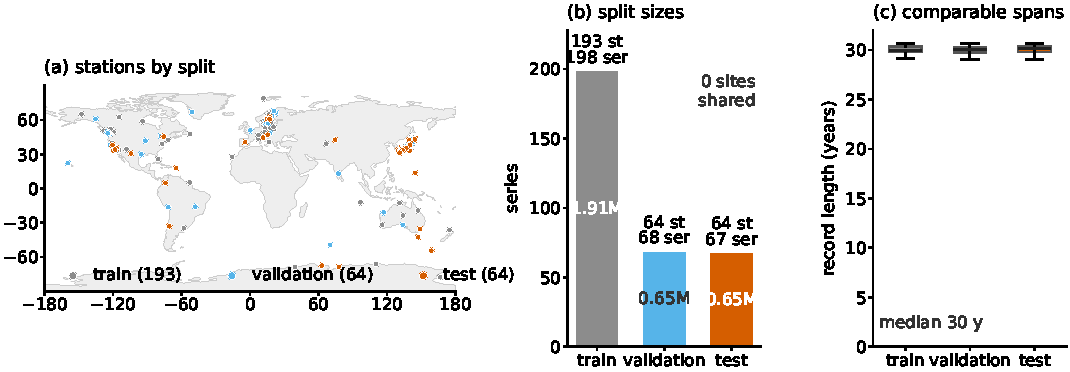
\includegraphics[width=\linewidth]{figures/fig04_split.pdf}
\caption{The split is drawn by site, not by epoch. (a) Held-out sites cover all
five regions and both analysis centres; (b) the three folds hold 193, 64 and 64
sites (198, 68 and 67 series) with zero sites shared; (c) the folds have
comparable record lengths (median about 30 years). Because every series of a
site stays in one fold, a learned method cannot memorise a station in training
and be scored on another component or source of the same station.}
\label{fig:split}
\end{figure}

\paragraph{Real discontinuity labels.}
For the real-label detection task we use the NGL discontinuity catalogue
(\url{https://geodesy.unr.edu/NGLStationPages/steps.txt}, downloaded
2026-10-18; 142\,625 lines; catalogue sha256
\texttt{\seqsplit{49894f7566ed34da3eb646087fc2fc64c5766720ba2368a3f6f6df53f3f282d8}}).
Two codes are retained: code 1, equipment change, and code 2, possible earthquake
step. A label is kept for a component only when its catalogued date lies inside
the record with a 0.5-year margin, its observed level change is at least three
times the local noise scale, and no other kept label lies within 60 days. This
yields 1\,743 labels on 153 component series from 58 held-out stations. The
labels are dominated by code 2 (1\,691 of 1\,743), so the real-label task
measures detection of earthquake-related steps more than of equipment changes;
we state this as a property of the data, not as a claim about all offsets. The
catalogue dates are not adjusted for post-seismic transients, which contributes
to the detection delay measured in Sec.~\ref{sec:results:t3:real}.

\paragraph{External and regional arms.}
Held-out JPL sites form the external arm: the six test JPL series are scored
separately from the 61 NGL series by the same methods. As a regional check we
also group the test sites into five geographic regions (Europe, North America,
Asia, Pacific and other) and report per-region scores (Fig.~\ref{fig:map}).
Neither arm changes any training or threshold decision.

\begin{figure}[t]
\centering
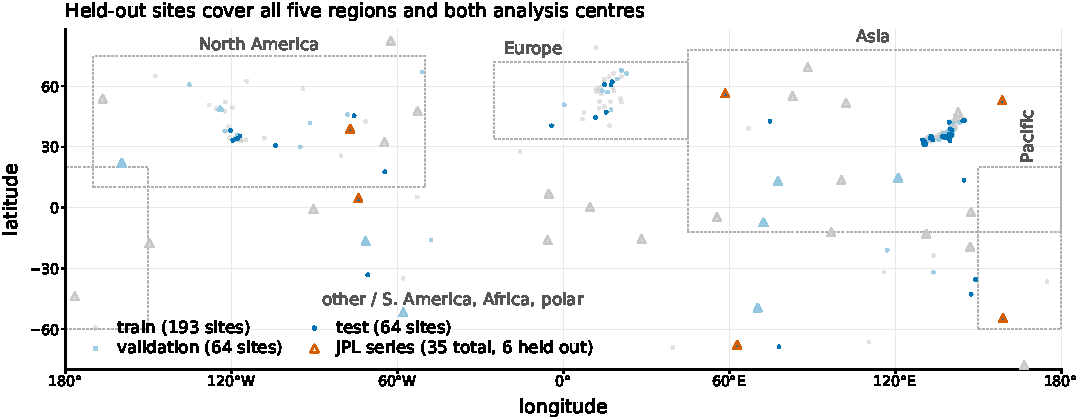
\includegraphics[width=\linewidth]{figures/fig11_map.pdf}
\caption{Geographic coverage of the split. Held-out (orange) sites fall in all
five scoring regions and include both NGL and JPL series, so the regional and
external arms test the same frozen networks outside the training geography
rather than a single continent. The map is descriptive; it enters no training or
threshold decision.}
\label{fig:map}
\end{figure}

\paragraph{Noise levels.}
The injected noise in the primary experiments is white noise with
$\sigma_{\rm WN}=1.5$~mm plus flicker noise with $\sigma_{\rm FN}=3.0$~mm. The
random-walk arm adds $\sigma_{\rm RW}=1.0$~mm. These levels were fixed before
any task was run. As a check on where they sit, we applied Whittle MLE to the
robust trajectory residual of all 999 component series in the benchmark: the
median white-noise level is 1.90~mm (interquartile range 1.39--3.67) and the
median flicker level 2.26~mm (1.61--5.74). The injected white level therefore
lies near the lower quartile and the flicker level inside the central half of
the empirical distribution (Fig.~\ref{fig:station_noise}). The recovered
random-walk median is 10.29~mm\,yr$^{-1/2}$, but that estimate absorbs
unmodelled transients and is an upper bound; the injected 1.0~mm\,yr$^{-1/2}$
is below it, so the random-walk arm is a sensitivity test rather than a
calibrated replay of the stations' noise.

\begin{figure}[t]
\centering
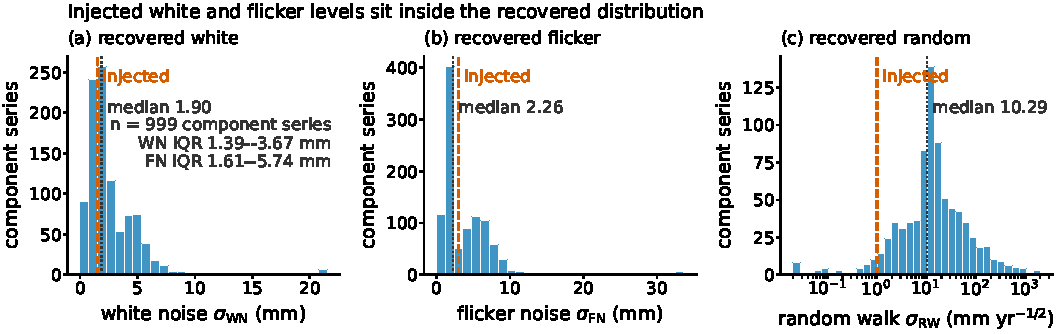
\includegraphics[width=\linewidth]{figures/fig14_station_noise.pdf}
\caption{Whittle estimates on the robust residual of every benchmark series.
The recovered white-noise distribution has a median of 1.90~mm (interquartile
range 1.39--3.67) and the recovered flicker distribution a median of 2.26~mm
(1.61--5.74); the injected levels (1.5 and 3.0~mm, dashed) sit near the lower
quartile and inside the central half, respectively. The random-walk estimate is
an upper bound because transients are absorbed by that component, which is why
the random-walk arm is a sensitivity test.}
\label{fig:station_noise}
\end{figure}


\section{Methodology}
\label{sec:method}

The three tasks share one signal model, one noise model and one scoring harness,
and every method is scored on the same realisation. The protocol differs from
the first version in two places: the truth is drawn from two families, one inside
and one outside the parametric basis, and detection is additionally scored
against real catalogue labels. Table~\ref{tab:methods} collects the methods and
their costs; the text gives only what the table cannot. Fig.~\ref{fig:pipeline}
shows how the stages connect: the same frozen realisation feeds every candidate,
and every candidate is carried through to the velocity product.

\subsection{Signal and noise model}
\label{sec:method:model}

A coordinate component is modelled as
\begin{equation}
y(t) = x(t) + \varepsilon(t), \qquad t\in[t_0,t_0+T],
\label{eq:obs}
\end{equation}
on a daily grid ($\Delta t=1/365.25$~yr), with
\begin{equation}
\label{eq:signal}
\begin{aligned}
x(t) =\;& v\,(t-t_0)
+ S_1\bigl[1+a_m\sin(2\pi f_m(t-t_0)+\phi_m)\bigr]
\sin(2\pi(t-t_0)+\phi_1) \\
&+ S_2\sin(4\pi(t-t_0)+\phi_2)
+ \sum_k b_k H(t-e_k) \\
&+ \sum_j c_j H(t-e_j)e^{-(t-e_j)/\tau_j},
\end{aligned}
\end{equation}
where $H$ is the Heaviside step and $v$ is the secular velocity. The stochastic
term is power-law noise with spectral density
\begin{equation}
S(f)=\sigma_{\rm WN}^2+\sigma_{\rm FN}^2\Bigl(\frac{f_0}{f}\Bigr)
+\sigma_{\rm RW}^2\Bigl(\frac{f_0}{f}\Bigr)^2,
\label{eq:psd}
\end{equation}
generated by inverse Fourier synthesis on a fixed frequency grid. The primary
experiments set $\sigma_{\rm WN}=1.5$~mm and $\sigma_{\rm FN}=3.0$~mm with
$\sigma_{\rm RW}=0$; the random-walk arm adds $\sigma_{\rm RW}=1.0$~mm.

\subsection{Ground-truth protocol}
\label{sec:method:inject}

The deterministic signal is never known on a real station, so it is created by
injection. Two families are used for every denoising and gap-filling score.

\emph{In-family.} The trend and harmonic amplitudes of Eq.~\eqref{eq:signal} are
taken from a robust fit of the real series, with a mild amplitude modulation
($a_m=0.35$). This is the family the trajectory model assumes, up to the
modulation.

\emph{Out-of-family.} The same station fit is used for the trend and mean
amplitudes, but the annual term receives strong multi-year modulation
($a_m\in[0.6,1.0]$), one or two long-lived exponential transients with decay
times of 0.3--1.5 years are added, and a logarithmic post-seismic relaxation is
included for some stations. These structures cannot be represented by constant
harmonics. The truth is still the deterministic part, so recovery error remains
exact.

Both families are also realised on a fully synthetic grid that sweeps the
parameters beyond what the station set contains. The learned models are always
scored by the network trained on the matching family, so an out-of-family score
is not an artefact of testing an in-family network on unfamiliar structure.

\paragraph{Tasks.}
\emph{T1 denoising} leaves $y$ intact and asks for $\hat{x}$. \emph{T2 gap
filling} removes contiguous blocks of $L\in\{5,10,30,60,120,365\}$ days and asks
for the missing values. \emph{T3 offset detection} adds offsets of amplitude
$A\in\{2,4,8,16,25\}$~mm at epochs at least two years apart and asks for the
epoch list; the real-label arm instead uses the catalogue epochs of
Sec.~\ref{sec:data}. For the real-label arm the match tolerance is 180 days to
allow for catalogue dates that refer to the earthquake rather than to the
observable break, and the minimum separation is 60 days; synthetic detection uses
a 30-day tolerance and 45-day separation, because its truth is exact.

\subsection{Methods}
\label{sec:method:methods}

Table~\ref{tab:methods} lists the classical and learned arms. All classical
methods are deterministic given $(t,y)$ and are fitted on the data they are
applied to. The trajectory model is an iteratively reweighted robust fit of trend
plus constant annual and semiannual harmonics. The Kalman/RTS smoother uses the
same basis with a small process noise. SSA embeds the series in a Hankel matrix
and reconstructs from its leading components; gap filling uses the iterative
variant. Wavelet shrinkage uses a db4 transform and soft thresholding at the
VisuShrink level. Interpolators are piecewise linear and shape-preserving cubic
(PCHIP); a natural cubic spline is not used because it overshoots multi-week gaps.
The classical detector is a greedy two-sample scan of the robust residual: the
epoch with the largest standardised step is accepted, its neighbourhood is
suppressed, the design is augmented, and the search repeats until the statistic
falls below threshold. To put both detector families on the same footing, both
are reduced to a decision field (the classical step statistic and the network
output) and read out by the same threshold-plus-minimum-separation rule; this
allows full precision--recall curves rather than a comparison of two hand-tuned
operating points.

\paragraph{Learned arms.}
The primary network is a one-dimensional U-Net with a contracting encoder and
an expanding decoder, skip connections and $2^3$-fold pooling (base width 12, depth 3,
213\,385 parameters; Fig.~\ref{fig:unet}); one network is trained per task. The
second architecture is a temporal convolutional network with residual blocks,
kernel width 5, channel widths 40--80 and dilations 1, 2, 4, 8 and 16, giving
227\,537 parameters. Both are trained under the identical generator, budget
(3000 steps, batch 32, learning rate $2\times10^{-3}$), window length (1024 days)
and seed list, so architecture and seed effects are not confounded with training
protocol. Denoising and gap filling use ten seeds for each architecture;
detection uses twenty U-Net seeds and ten TCN seeds. A small bidirectional GRU
from the first version (four seeds) is reported only as a sensitivity check.

\begin{figure}[t]
\centering
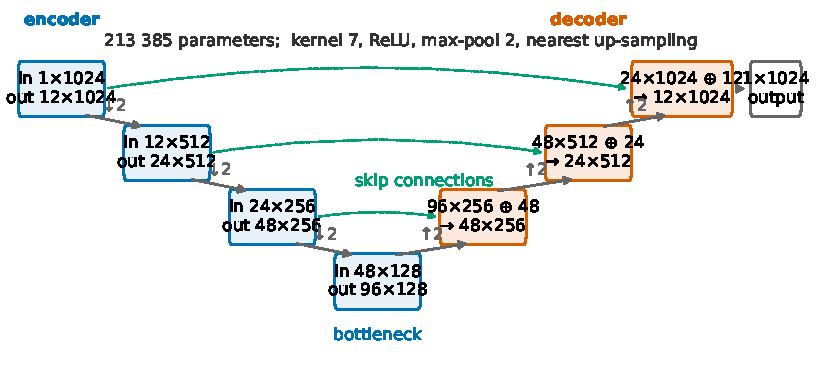
\includegraphics[width=\linewidth]{figures/fig03_unet.pdf}
\caption{The one-dimensional U-Net scored in the primary learned arm. Three
encoder stages halve the resolution and double the width (12 to 96 channels),
the decoder restores it with nearest-neighbour up-sampling, and skip connections
carry the fine-scale detail across the bottleneck. The network has 213\,385
parameters and is trained separately for each task.}
\label{fig:unet}
\end{figure}

Training draws a fresh window at every step. Inputs and targets are standardised
by robust per-window statistics; the detector additionally high-passes the input
and divides by a robust noise scale, so offset amplitude enters as a
signal-to-noise ratio. Long series are processed with 50\% overlapping windows
and averaged. At scoring time each window is standardised by its own statistics
and the network output is transformed back with the same statistics, so the
normalisation at inference matches the one used in training. The whole-series
normalisation of the first version is kept only as an ablation. The gap filler receives the observation mask as a second input
channel. The training distribution covers gaps of 5--120 days, offset amplitudes
in $[-12,12]$~mm and $\sigma_{\rm WN}\in[0.5,3]$~mm,
$\sigma_{\rm FN}\in[0,5]$~mm; the 365-day gap and the 16--25~mm amplitudes are at
or beyond that support and are read as extrapolation.

\begin{table*}[t]
\centering
\caption{Methods compared. ``Field'' denotes the decision field used for
detection; cost is per series unless stated. Parameter counts are for the
learned models; training wall-clock is for one seed on one V100.}
\label{tab:methods}
\footnotesize
\setlength{\tabcolsep}{2.5pt}
\begin{tabularx}{\textwidth}{@{}p{2.05cm}p{1.45cm}Xp{2.2cm}p{1.4cm}p{2.0cm}@{}}
\toprule
Method & Class & Key assumption & Input $\to$ output & Cost & Reference \\
\midrule
Trajectory MLE & parametric & trend + constant harmonics, power-law noise & $y\to\hat{x}$; velocity, $\sigma_v$ & closed form, $<$1~s & \citet{williams2003coloured} \\
Kalman/RTS & parametric & harmonic state, small process noise & $y\to\hat{x}$ & $<$1~s & \\
SSA & model-free & low-rank Hankel structure & $y\to\hat{x}$; gap fill & $<$1~s & \citet{wdowinski1997spatial,ji2024ssa} \\
Wavelet & model-free & sparsity in db4 domain & $y\to\hat{x}$ & $<$1~s & \citet{ji2020wavelet} \\
Moving median & model-free & local smoothness & $y\to\hat{x}$ & $<$1~s & \\
Linear/PCHIP & interp. & local continuity & $y$, mask $\to\hat{x}$ & $<$1~s & \\
Step scan & hyp.\ test & piecewise-constant level & $y\to$ epochs & $<$1~s & \citet{gazeaux2013detecting} \\
U-Net & learned & convolutional encoder--decoder & $y$(+mask) $\to\hat{x}$ or field & 213\,385; 8~min & \citet{ronneberger2015unet} \\
TCN & learned & dilated temporal convolutions & $y$(+mask) $\to\hat{x}$ or field & 227\,537; 6~min & \citet{bai2018tcn} \\
BiGRU & learned & recurrent encoder--decoder & $y\to\hat{x}$ & 182\,785; 5.1~h & \\
\bottomrule
\end{tabularx}
\end{table*}

\subsection{Metrics}
\label{sec:method:metrics}

For T1 the error is $\mathrm{RMSE}(\hat{x},x)$ and the reported quantity is the
reduction $1-\mathrm{RMSE}/\mathrm{RMSE}_{\rm none}$ relative to the undenoised
series. For T2 the error is the RMSE at the masked epochs against the withheld
observation $y$, the value the station recorded; where stated we also report the
error against the noise-free signal $x$, which separates recovering the signal
from reproducing correlated noise. For T3, predicted epochs are greedily matched
to true epochs within the task tolerance, and precision, recall, $F_1$ and average
precision follow. Detection delay is the signed difference between the matched
prediction and the true epoch.

\subsection{Downstream propagation}
\label{sec:method:downstream}

For every method we fit the velocity on its output with the same estimator: the
trend coefficient of the robust trajectory fit and its generalised-least-squares
covariance under a power-law spectrum \citep{williams2008cats,bos2008fast},
\begin{equation}
\hat v=(X^\top C^{-1}X)^{-1}X^\top C^{-1}y,\qquad
\hat\sigma_v^2=\bigl[(X^\top C^{-1}X)^{-1}\bigr]_{vv},
\label{eq:downstream}
\end{equation}
with the WN, FN and RW amplitudes obtained by Whittle maximum likelihood on the
periodogram. Two covariance arms are computed. In the primary (raw-noise) arm the
noise amplitudes are estimated once on the untreated series and held fixed for
every method, so the methods differ only in the series they hand to the velocity
fit. In the secondary (naive) arm the noise is re-estimated on each method's
output; this is the protocol of the first version, and it fails for
model-based denoisers because their output retains no residual from which a
noise amplitude can be recovered. Because the injected velocity is known, the
empirical scatter of $\hat v$ across realisations is compared with the median
reported $\hat\sigma_v$. Their ratio is the calibration ratio (one is honest,
below one is optimistic), and we also report the empirical coverage of the
nominal one- and two-sigma intervals. The random-walk arm repeats the whole chain
with $\sigma_{\rm RW}=1.0$~mm\,yr$^{-1/2}$ and a three-component noise model.


\section{Results}
\label{sec:results}

Every comparison below scores the same held-out realisations with the same
metrics. Learned methods are scored only on stations the network never saw, and
each learned number is a distribution over training seeds rather than one draw.
Section~\ref{sec:results:check} shows that the harness recovers a known truth,
Sections~\ref{sec:results:t1}--\ref{sec:results:t3} give the three tasks, and
Sections~\ref{sec:results:downstream}--\ref{sec:results:external} follow the
products downstream.

\subsection{Validation of the injection and estimation pipeline}
\label{sec:results:check}

On a synthetic grid that sweeps white and flicker amplitudes, the recovered
white-noise level departs from the injected one by at most $0.0197$ in relative
terms and the flicker level shows a median relative bias of $-0.0377$. The
flicker bias is the finite-length behaviour of Whittle estimation, shared by
all methods and therefore cancelling in comparisons. For a series with known
white and flicker noise of length $n=3650$ days, the Monte-Carlo scatter of the
estimated velocity is $0.1613$~mm\,yr$^{-1}$ against a median reported GLS
uncertainty of $0.1615$~mm\,yr$^{-1}$, a calibration ratio of $1.0011$. The
estimator is calibrated to better than $0.1\%$ on the uniform grid. On the
irregularly sampled test stations the untreated series is itself below nominal
coverage (Sec.~\ref{sec:results:downstream}), so the downstream calibration is
read as a relative comparison between methods, not as an absolute statement
about geodetic uncertainty.

Figure~\ref{fig:station_noise} applies the same estimator to every benchmark
series. The recovered white and flicker levels bracket the injected 1.5 and
3.0~mm, while the recovered random walk is an upper bound because transients are
absorbed by that component.

\subsection{Task 1: denoising}
\label{sec:results:t1}

Denoising is scored as the reduction $1-\mathrm{RMSE}(\hat S,S)/\mathrm{RMSE}(y,S)$
on the same realisations, where $y$ is the noisy series and $S$ the truth.
Figure~\ref{fig:truth_families} shows the construction of the two families and
the per-station scores.

\begin{figure}[t]
\centering
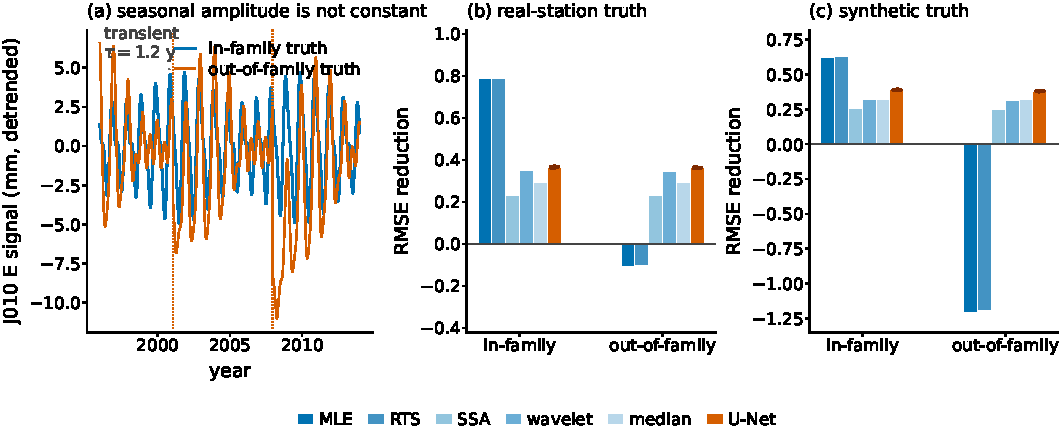
\includegraphics[width=\linewidth]{figures/fig08_truth_families.pdf}
\caption{Parametric denoising depends on the truth family; the learned one does
not. (a) The out-of-family truth modulates the annual amplitude, adds exponential
transients (dotted epochs) and a logarithmic relaxation; the in-family truth
keeps the amplitude nearly constant. (b) On real-station truth the trajectory
model and RTS smoother dominate in-family and fall below zero out-of-family,
whereas the U-Net stays between $0.363$ and $0.366$ and sits above every
model-free decomposition in both families. (c) The fully synthetic grid shows the same
pattern. Bars are means over realisations, orange dots are individual training
seeds, and classical methods are deterministic.}
\label{fig:truth_families}
\end{figure}

On the in-family truth, where the signal is the trend--harmonic trajectory fitted
to a real station, the parametric estimator reproduces its earlier result: the
trajectory model reduces the error by $0.790$ (95\% bootstrap interval
$0.776$--$0.804$) and the Kalman/RTS smoother by $0.791$. The model-free
decompositions follow at a distance: wavelet $0.349$, moving median $0.293$, SSA
$0.232$. The U-Net, scored with the per-window normalisation used in training,
reaches $0.366 \pm 0.002$ over ten seeds. It does not reach the parametric
estimators, which see the correct basis, but it is above every model-free
decomposition in the same regime.

The out-of-family truth keeps the same stations but adds a multiplicative
seasonal modulation, exponential transients and logarithmic post-seismic
relaxation. The trajectory model falls to $-0.106$ (interval $-0.434$ to
$0.181$) and the RTS smoother to $-0.104$: with this truth the fit can leave the
series noisier than it found it. The model-free methods barely move (wavelet
$0.345$, median $0.292$, SSA $0.231$), because none of them assumes a stationary
harmonic basis. The U-Net, trained on the out-of-family generator, is almost
unchanged at $0.363 \pm 0.001$ and is now the strongest method apart from the
untreated series.

The fully synthetic regimes make the same point with more realisations.
In-family, the trajectory model reduces the error by $0.624$ and the U-Net by
$0.389 \pm 0.001$; the moving median reaches $0.320$, the wavelet $0.317$ and
SSA $0.252$. Out-of-family, the trajectory model drops to $-1.211$ while the
U-Net stays at $0.381 \pm 0.001$, against $0.318$ for the median and $0.312$ for
the wavelet. The learned denoiser therefore overtakes the model-free
decompositions in all four regimes, on both the real-station and the fully
synthetic truth, and its score changes by less than $0.01$ when the truth family
changes. The denoising conclusion is conditional only on the parametric
alternative: the trajectory model wins by more than a factor of two when the
truth lies in its basis and adds error when it does not, while the learned
denoiser is the best non-parametric choice in both families.

The difference from the first version comes from the inference protocol, not
from the truth construction. Scoring the same networks on whole-series
normalisation returns $0.193$ in-family and $0.274$ out-of-family, which is why
the earlier draft placed the U-Net below SSA on real stations. Matching the
normalisation to the training windows removes that gap and leaves the ordering
above.

\subsection{Task 2: gap filling}
\label{sec:results:t2}

Gap filling is scored on 40 held-out component series of long synthetic records
and on 30 held-out component series of real stations, with gaps of 5, 30 and 120
days. Two inference modes are reported for the network: whole-series
normalisation, the protocol of the first version, and per-window normalisation,
which matches the statistics under which the network was trained.

On long synthetic records (Table~\ref{tab:t2}), the 5-day gap is filled best by
SSA ($2.57$~mm), followed by linear interpolation ($2.69$) and the per-window
U-Net ($2.80 \pm 0.06$); the trajectory model is at $3.41$. At 30 days the order
changes: the per-window U-Net reaches $3.07 \pm 0.03$ and beats linear
interpolation ($3.34$), SSA ($3.37$), PCHIP ($3.59$) and the trajectory model
($3.79$). At 120 days the trajectory model is best ($3.99$), the per-window
U-Net reaches $5.09 \pm 0.08$, and whole-series inference fails at
$7.59 \pm 0.26$.

\begin{table}[t]
\centering
\caption{Gap-filling error (RMSE at the missing days, mm) for long synthetic
series ($n=40$ component series) and real held-out stations ($n=30$). The
per-window U-Net is the best method at 30-day gaps on both record sets, but the
real-set margin does not survive the full 201 component series
(Sec.~\ref{sec:results:external}); the trajectory model is best at 120 days,
and the whole-series arm fails. Values for
the network are means over ten training seeds with the seed standard deviation.}
\label{tab:t2}
\setlength{\tabcolsep}{3pt}
\begin{tabular}{lccccc}
\hline
 & \multicolumn{3}{c}{Long synthetic} & \multicolumn{2}{c}{Real stations} \\
\cmidrule(lr){2-4}\cmidrule(lr){5-6}
Method & 5~d & 30~d & 120~d & 5~d & 30~d \\
\hline
Linear         & 2.69 & 3.34 & 4.72 & 2.65 & 2.93 \\
PCHIP          & 2.80 & 3.59 & 5.22 & 2.76 & 3.10 \\
SSA            & 2.57 & 3.37 & 4.73 & 2.51 & 2.97 \\
Trajectory MLE & 3.41 & 3.79 & 3.99 & 3.16 & 3.35 \\
\hline
U-Net, whole series & $4.52 \pm 0.54$ & $3.55 \pm 0.14$ & $7.59 \pm 0.26$ & $9.98 \pm 1.80$ & $6.16 \pm 0.60$ \\
U-Net, per window   & $2.80 \pm 0.06$ & $3.07 \pm 0.03$ & $5.09 \pm 0.08$ & $2.55 \pm 0.03$ & $2.74 \pm 0.03$ \\
\hline
\end{tabular}
\end{table}

The real stations reproduce the same pattern (Table~\ref{tab:t2}). At 5 days SSA
($2.51$~mm) and the per-window U-Net ($2.55 \pm 0.03$) are tied, with linear
interpolation at $2.65$; at 30 days the per-window U-Net leads at
$2.74 \pm 0.03$ against $2.93$ for linear interpolation and $2.97$ for SSA. The
whole-series arm is not competitive at either length ($9.98 \pm 1.80$ and
$6.16 \pm 0.60$), up to a factor of four worse than the same network evaluated
per window. The gap-filling failure reported in the first version was therefore
an inference-normalisation defect, not an inability of the architecture to
interpolate. With the defect removed, the learned imputer leads at 30-day gaps
on synthetic records and on this 30-series real subset, but not across the full
held-out set (Sec.~\ref{sec:results:external}); it loses at 5 days by a small
margin and at 120 days by a large one. Fig.~\ref{fig:impute_log} shows the same scores on a log
scale, with seed error bars. The per-window curve rises by at most $0.3$~mm
between 5 and 30 days, while the whole-series arm is $1.7$~mm above it at 5 days
on the synthetic records and $7.4$~mm above it on the real stations.

\begin{figure}[t]
\centering
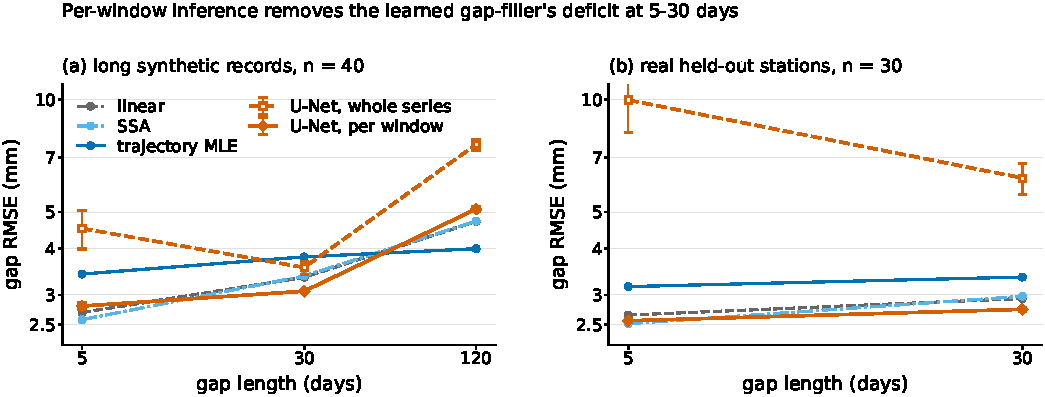
\includegraphics[width=\linewidth]{figures/fig06_impute_log.pdf}
\caption{Gap-filling error against gap length. Per-window inference (solid
orange, diamonds) is within 0.1~mm of SSA at 5 days and best at 30 days on both
long synthetic records (a) and real held-out stations (b); the trajectory model
remains best at 120 days. The whole-series arm (dashed, open squares) is not a
competitive configuration at any length. Error bars are one standard deviation
over ten training seeds; classical methods are deterministic and carry none.}
\label{fig:impute_log}
\end{figure}

The trajectory model's advantage at long gaps is visible in signal error rather
than observation error: against the missing true signal, its RMSE is $0.74$~mm
at 5 days, $0.68$ at 30, $0.78$ at 120 and $0.78$ at 365 days, while the
whole-series network reaches $11.40$, $5.97$, $10.26$ and $61.0$~mm at the same
lengths. That arm is the defective configuration, and we do not extrapolate the
30-day per-window win to year-long gaps, for which no per-window measurement was
made.

\subsection{Task 3: offset detection under a fair protocol}
\label{sec:results:t3}

Both detectors are reduced to a decision field, a threshold and a minimum
separation, so the comparison measures the field rather than a tuning accident.
Offsets of 2, 4, 8, 16 and 25~mm are injected at known epochs; a detection within
30 days counts as a match, and two accepted detections must be at least 45 days
apart. The threshold is selected per seed on held-out validation draws, which is
the protocol a user would follow, and we also report the oracle threshold.

At the validation-selected threshold the classical detector has the higher F1 at
every amplitude (Table~\ref{tab:t3}): $0.073$ against $0.0005$ at 2~mm, $0.259$
against $0.039$ at 4~mm, $0.815$ against $0.460$ at 8~mm, $0.963$ against
$0.709$ at 16~mm and $0.975$ against $0.725$ at 25~mm
(Fig.~\ref{fig:fair_detector}). The learned field nevertheless ranks large
steps better: its average precision is higher at 16~mm ($0.648$ against $0.208$)
and at 25~mm ($0.669$ against $0.007$). The two metrics answer different
questions. Average precision integrates over all thresholds and rewards a field
that orders events well; the deployed detector uses one threshold, and there the
classical field is better. Reporting only average precision would have hidden
that its operating point is worse.

\begin{figure}[t]
\centering
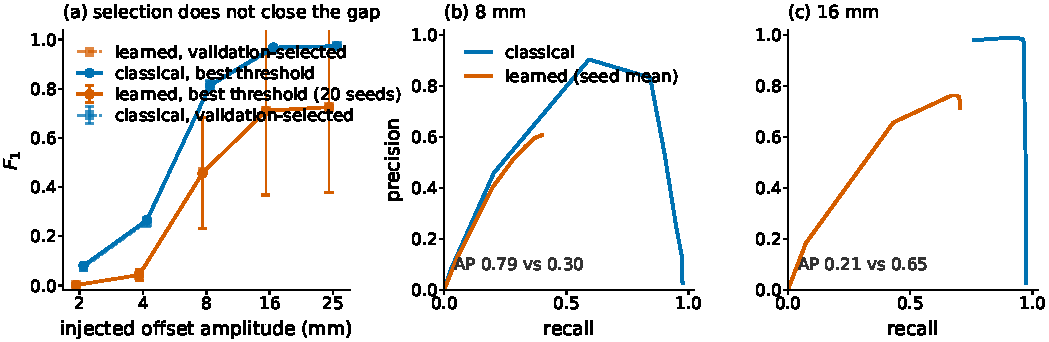
\includegraphics[width=\linewidth]{figures/fig13_fair_detector.pdf}
\caption{Threshold selection does not close the detection gap. (a) Validation-
selected and oracle $F_1$ for the classical and learned fields: the learned
field improves when its threshold is tuned, but not enough to meet the classical
detector at any amplitude. (b),(c) Precision--recall curves at 8 and 16~mm: the
learned field has lower average precision at 8~mm and higher at 16~mm, which is
the ranking-versus-operating-point distinction in the text. The learned seed mean
is shown with one standard deviation; classical detection is deterministic.}
\label{fig:fair_detector}
\end{figure}

\begin{table}[t]
\centering
\caption{Synthetic offset detection by injected amplitude. The threshold is
selected on held-out validation draws for every seed. The learned field has
higher average precision at 16 and 25~mm, but at the operating point a user
would deploy its F1 is lower at every amplitude. Learned values are means over
twenty seeds; the F1 column also gives the seed standard deviation.}
\label{tab:t3}
\footnotesize
\setlength{\tabcolsep}{4pt}
\begin{tabular}{ccccc}
\hline
Amplitude (mm) & Classical AP & Classical F1 & Learned AP & Learned F1 \\
\hline
2  & 0.032 & 0.073 & 0.0000 & $0.0005 \pm 0.002$ \\
4  & 0.143 & 0.259 & 0.0028 & $0.0395 \pm 0.024$ \\
8  & 0.788 & 0.815 & 0.298  & $0.460 \pm 0.222$ \\
16 & 0.208 & 0.963 & 0.648  & $0.709 \pm 0.334$ \\
25 & 0.007 & 0.975 & 0.669  & $0.725 \pm 0.341$ \\
\hline
\end{tabular}
\end{table}

\subsection{Task 3 on real catalogue labels}
\label{sec:results:t3:real}

The NGL discontinuity catalogue supplies 1\,743 labels on 153 held-out component
series from 58 stations: 52 code-1 and 1\,691 code-2 entries, distributed over
1006 East, 528 North and 209 Up series. The labels are matched to the series,
restricted to the record span and to offsets whose observed amplitude exceeds
three times the local noise level, and deduplicated at 60 days. Amplitudes are
skewed (median $-6.23$~mm, interquartile range $-17.79$ to $11.61$~mm) and
concentrated in East, which is where the catalogue is densest. Stations, not
series, are split into validation and scoring halves over 40 draws, so a
detector never chooses a threshold on the stations it is scored on.

The classical detector reaches F1 $0.457 \pm 0.027$, average precision $0.322$,
precision $0.490$ and recall $0.536$. Recall rises with signal-to-noise ratio,
from $0.398$ in the 3--5 stratum to $0.610$ in 5--10 and $0.848$ above 10.
Its median signed delay is $-51.5$ days, with an absolute median of $69.7$ days.
The twenty U-Net seeds average F1 $0.232 \pm 0.107$ and average precision
$0.135$; precision is $0.329$ and recall $0.302$. Three seeds collapse to
essentially no detections (F1 $0.0000$, $0.0002$ and $0.0004$), which is why the
seed mean is far below the median seed ($0.290$). The best seed reaches $0.316$.
The ten TCN seeds average F1 $0.273 \pm 0.096$, average precision $0.173$,
precision $0.368$ and recall $0.356$, with one collapsed seed and a best seed of
$0.319$. The TCN is therefore the stronger of the two learned architectures on
every aggregate metric, and it is still the weaker detector: even its best seed
lies below the classical mean minus one standard deviation ($0.430$). Where a
U-Net seed does detect events, its absolute median delay is $16.5$--$52.1$ days
and its signed median lies between $-18.3$ and $+1.0$ days; the TCN range is
$7.8$--$39.9$ days, signed between $-4.8$ and $+0.7$ days. Matched learned
detections sit closer to the catalogued epoch than the classical ones, while the
classical detector finds more of them at lower precision.

Real labels are harder than synthetic ones for both detectors. The classical F1
falls from $0.815$ at 8~mm in the synthetic protocol to $0.457$ on the catalogue,
and the U-Net F1 from $0.460$ to $0.232$. The same classical advantage holds for
the TCN on the synthetic subset scored in Sec.~\ref{sec:results:arch}. Neither
learned architecture changes the ordering.
The regional split shows the same shortfall everywhere the catalogue is dense:
Asia, which supplies 39 of the 58 labelled stations, gives the classical
detector F1 $0.488$, the U-Net $0.251$ and the TCN $0.294$; North America gives
$0.426$, $0.230$ and $0.272$. Europe is the weakest region for every method
($0.267$, $0.101$ and $0.109$) and has only six labelled stations, so its
ranking is the least stable. The centre and region ordering is shared by the
classical and learned arms, which rules out a single-region artefact as the
explanation of the learned shortfall. Figure~\ref{fig:real_offsets} shows the
per-seed distribution, the signal-to-noise strata and the delay.

\begin{figure}[t]
\centering
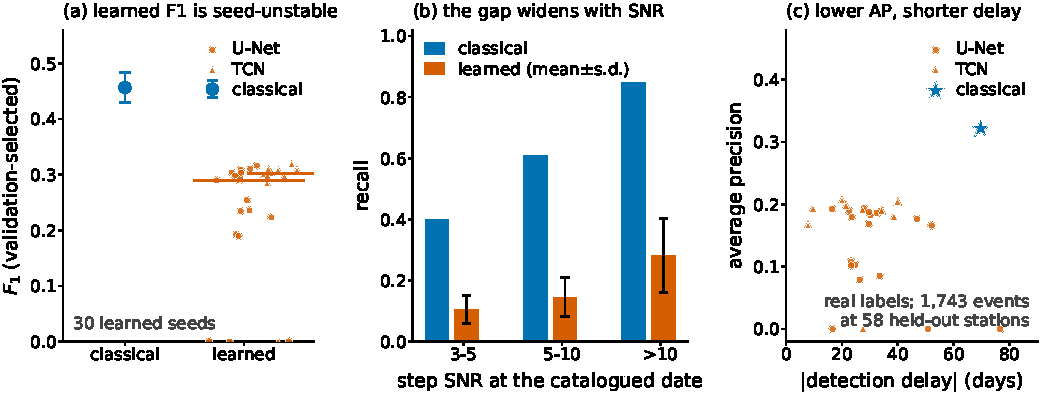
\includegraphics[width=\linewidth]{figures/fig09_real_offsets.pdf}
\caption{Detection against 1\,743 real catalogue labels. (a) The twenty U-Net
and ten TCN seeds spread from near-zero to just above the classical $F_1$, and
four seeds collapse; both learned means stay below the classical mean, and the
TCN mean is the higher of the two. (b) Recall rises with signal-to-noise ratio
for the classical detector, while the learned mean stays lower in every stratum.
(c) The learned fields have lower average precision but shorter matched delays;
they find fewer events, and the ones they find sit closer to the catalogued
epoch. Bars and points are seed statistics; the classical detector is
deterministic.}
\label{fig:real_offsets}
\end{figure}

\subsection{Downstream velocity and the random-walk arm}
\label{sec:results:downstream}

A benchmark product is only useful if the processed series yields a defensible
velocity. We therefore carry every method through the same GLS velocity fit on
six held-out stations and two components with three injected realisations each
(36 station--component--realisation draws per arm). Two noise models are used:
white plus flicker noise, and the same model with a random-walk component at
$\sigma_{\rm RW}=1.0$~mm\,yr$^{-1/2}$.

With white plus flicker noise, the trajectory MLE on the raw series has velocity
bias $-0.0024$~mm\,yr$^{-1}$ and RMSE $0.0586$~mm\,yr$^{-1}$. The classical
denoisers leave this essentially unchanged on the raw-noise arm: SSA $0.0588$,
RTS $0.0594$, moving median $0.0590$ and wavelet $0.0616$. The U-Net denoiser,
scored with training-matched per-window normalisation, reaches
$0.0605$~mm\,yr$^{-1}$ and a bias of $-0.0034$; its two seeds score
$0.0600$ and $0.0611$. At 30-day gaps the classical imputers are indistinguishable from the
complete series ($0.0581$--$0.0588$), and the U-Net imputer matches them at
$0.0586$. No method improves the velocity over the untreated series, but the
learned denoiser is no longer an outlier: it sits between the moving median and
the wavelet, $0.002$~mm\,yr$^{-1}$ behind the raw series.

That difference from the first version matters. Under whole-series
normalisation the same network produced $0.2087$~mm\,yr$^{-1}$; scoring it
window by window removes the mismatch and brings the velocity error back to the
level of the classical denoisers. The earlier negative downstream result was
therefore an inference-protocol artefact, not a property of learned denoising.

Calibration is quoted with the noise model estimated on the raw series and held
fixed for every method, because re-estimating the noise on a denoised output is
not a valid protocol: the trajectory and RTS outputs retain essentially no
residual, so a Whittle fit to them returns a near-zero noise level and a
vanishing reported uncertainty (calibration ratios $1.7\times10^{-14}$ and
$1.0\times10^{-6}$ in that arm). Against the raw-series noise model, the
reference reports a median velocity uncertainty of $0.0380$~mm\,yr$^{-1}$
against an empirical scatter of $0.0585$, a calibration ratio of $0.649$ and
1$\sigma$ coverage of $0.389$; classical denoisers stay between $0.618$ and
$0.647$, and the U-Net reaches $0.628$ with coverage $0.458$. The
under-coverage is the same irregular-sampling effect noted in
Sec.~\ref{sec:results:check}, which is why the ratios are comparable across
methods but should not be read as absolute geodetic uncertainties.

\begin{sloppypar}
Adding the random-walk component degrades the reference modestly and changes no
ordering. The raw/MLE bias moves from $-0.0024$ to $-0.0089$~mm\,yr$^{-1}$,
the RMSE from $0.0586$ to $0.0690$, the calibration ratio from $0.649$ to
$0.575$ and the 1$\sigma$ coverage stays at $0.389$. The classical denoisers
move to $0.0686$--$0.0713$; the U-Net denoiser reaches $0.0698$ with
calibration $0.570$ and coverage $0.403$, and the U-Net imputer $0.0690$ with
calibration $0.575$ and coverage $0.417$. The learned arms again track the
reference and the classical denoisers.
\end{sloppypar}
Fig.~\ref{fig:calibration} collects the calibration and coverage pairs, and
Fig.~\ref{fig:rw_effect} isolates the random-walk increment. The downstream
evidence is neutral: under the protocol-matched inference, neither learned arm
improves the velocity or its uncertainty, and neither destroys them.

\begin{figure}[t]
\centering
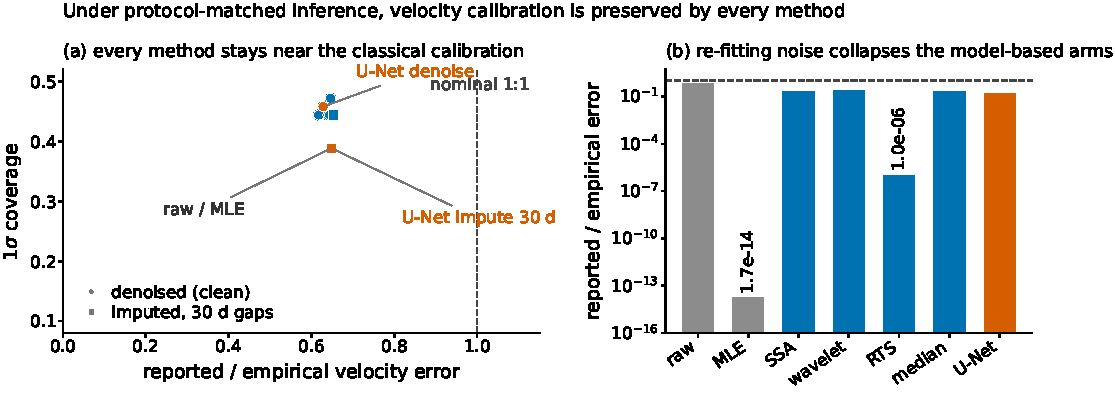
\includegraphics[width=\linewidth]{figures/fig07_calibration.pdf}
\caption{Protocol-matched inference keeps velocity calibration for every
method. (a) Reported uncertainty against empirical scatter for the clean arm:
the untreated series, the classical denoisers and both learned arms sit between
$0.62$ and $0.65$ with $1\sigma$ coverage of $0.39$--$0.47$; the learned
denoiser reaches $0.628$ and $0.458$. (b) Re-estimating the noise on each
output collapses the reported uncertainty for the trajectory MLE and the RTS
smoother ($1.7\times10^{-14}$ and $1.0\times10^{-6}$), because their residual is
nearly empty; the remaining methods stay within a factor of five of nominal.
That collapse is an artefact of the protocol, not a property of the method. The
vertical distance to the nominal line is the calibration error.}
\label{fig:calibration}
\end{figure}

\begin{figure}[t]
\centering
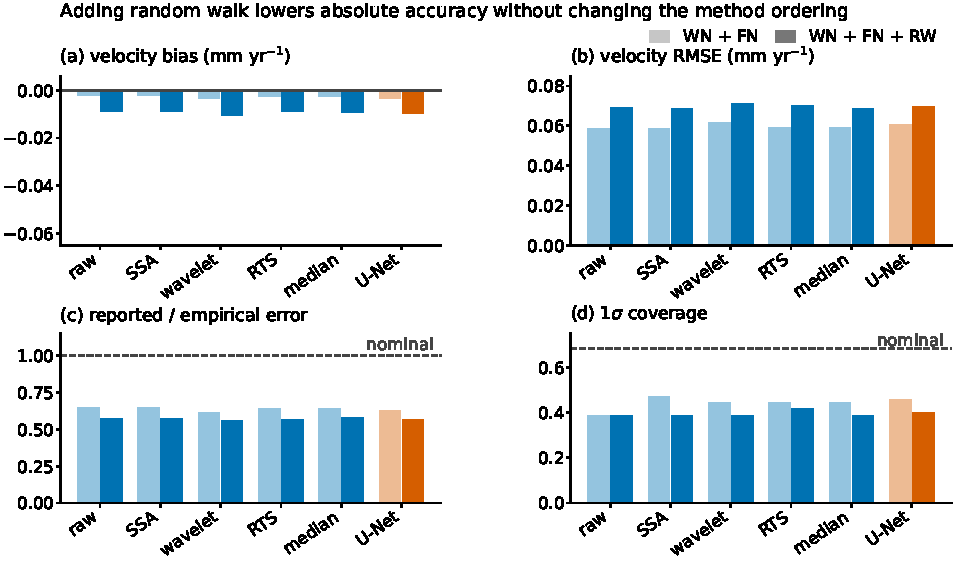
\includegraphics[width=\linewidth]{figures/fig12_rw_effect.pdf}
\caption{Adding a random-walk component changes the level, not the ordering.
Paired bars compare the white-plus-flicker arm (pale) with the white-plus-
flicker-plus-random-walk arm (solid) for velocity bias, velocity RMSE,
calibration ratio and $1\sigma$ coverage. Every method loses absolute accuracy
under the random-walk model (RMSE rises by about $0.010$~mm\,yr$^{-1}$) and
calibration falls from about $0.65$ to $0.57$; the ordering is unchanged and the
learned arms track the classical ones. Horizontal lines mark zero bias, the
nominal calibration ratio of one and the nominal $1\sigma$ coverage of $0.683$.}
\label{fig:rw_effect}
\end{figure}

\subsection{External and regional validation}
\label{sec:results:external}

The scores above come from the ten-station real subset and the thirty-series
long-record subset. To check whether they are a property of the benchmark or of
those subsets, we score every held-out test series under the same per-window
protocol: 67 series, 201 component series, of which 183 are NGL and 18 JPL,
split into Europe (18), North America (30), Asia (123), Pacific (24) and other
(6). Each component series receives three injected realisations and the ten
denoising and ten gap-filling checkpoints. No network is retrained and no
threshold is chosen, so the arm is descriptive: it asks whether the ranking
transfers, not whether a JPL-trained network would do better.

Denoising transfers. The U-Net removes $0.360 \pm 0.003$ on NGL and
$0.345 \pm 0.005$ on JPL, against $0.341$ and $0.317$ for the wavelet, $0.291$
and $0.322$ for the moving median and $0.230$ and $0.254$ for SSA. The
trajectory MLE stays ahead at $0.775$ and $0.665$. The learned denoiser is above
every model-free decomposition in both centres, and across the five regions its
mean lies between $0.333$ and $0.366$, against $0.700$--$0.812$ for the MLE and
$0.299$--$0.360$ for the wavelet. The one exception is Europe, where the U-Net
($0.358$) and the wavelet ($0.360$) are within $0.002$ of each other. The
denoising conclusion of Sec.~\ref{sec:results:t1} therefore does not depend on
the subset used to measure it.

Gap filling does not transfer as cleanly. On NGL the U-Net reaches
$2.964 \pm 0.034$~mm and linear interpolation $2.967$ [2.914, 3.017], with SSA at
$3.000$ and the MLE at $3.252$: a tie. On JPL the U-Net reaches
$3.293 \pm 0.042$ against $3.233$ [3.056, 3.416] for linear interpolation, with
SSA at $3.309$ and the MLE at $3.367$: the learned arm is $0.06$~mm behind. The
$2.74$~mm score of Sec.~\ref{sec:results:t2} came from a 30-series real subset;
on the full 201 component series the 30-day advantage is a tie on the NGL
majority and is absent on JPL. The regional split repeats the pattern: the U-Net
is the best filler in Asia ($2.990$ against $2.994$) and Europe ($2.910$ against
$3.028$), but linear interpolation is better in North America ($2.942$ against
$2.954$), the Pacific ($2.986$ against $3.089$) and the residual group ($3.068$
against $3.113$). The differences are at most $0.12$~mm, and
they do not support a product-level claim for learned gap filling on real data.
Fig.~\ref{fig:external} shows both tasks by centre and by region.

\begin{figure}[t]
\centering
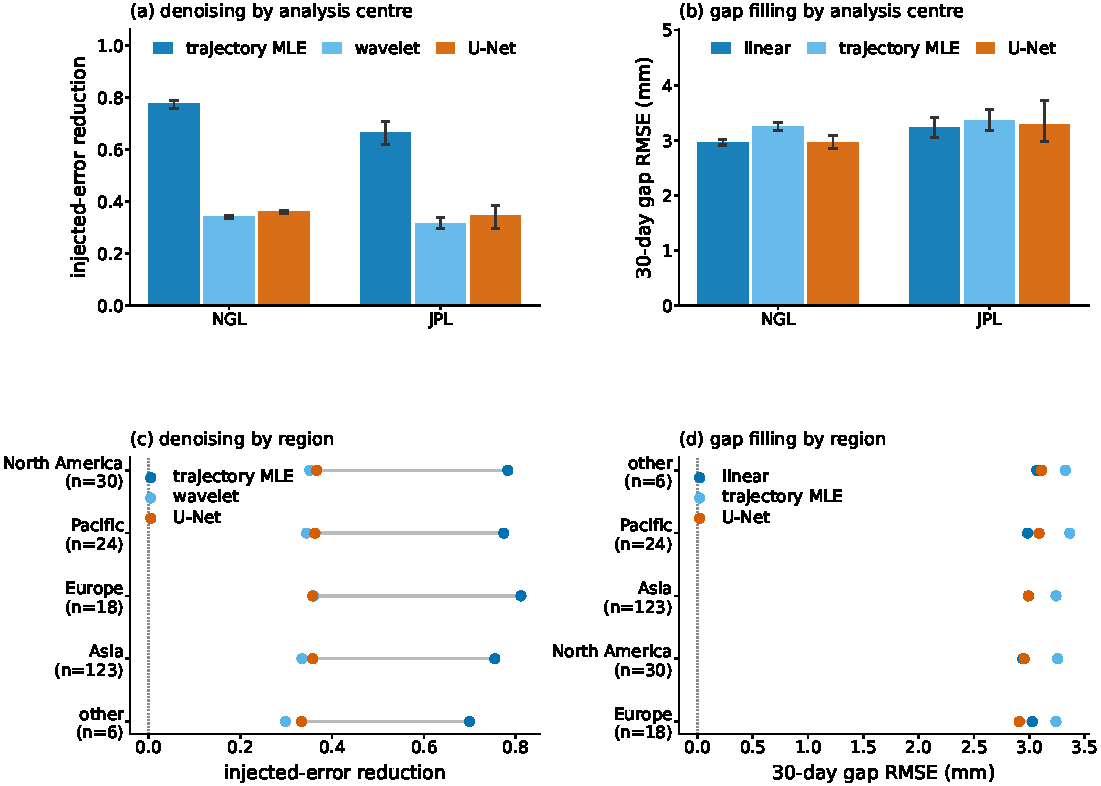
\includegraphics[width=\linewidth]{figures/fig15_external_regional.pdf}
\caption{The denoising ranking transfers across centres and regions; the
30-day gap-filling advantage does not. (a) Denoising and (b) 30-day gap filling
by analysis centre (NGL, JPL). (c)--(d) The same scores by region. Bars and
points are means over component series, with 95\% bootstrap intervals over
series for the classical methods; the learned value is the mean over ten
checkpoints and its seed standard deviation is smaller than the marker. The
learned denoiser stays above every model-free decomposition at both centres,
while the learned imputer ties linear interpolation on NGL and falls behind it
on JPL.}
\label{fig:external}
\end{figure}

\subsection{Architecture and seed variation}
\label{sec:results:arch}

The ranking is not a property of one architecture. Three learned families are
scored on the shared test split under one protocol: the U-Net (ten seeds for
denoising and gap filling, twenty for detection), the TCN (ten seeds per task)
and the smaller BiGRU of the first version (four seeds for denoising and gap
filling). Denoising and gap filling use ten held-out stations; detection uses
eight stations with one realisation, so its absolute levels are not comparable
with the twelve-station table above, only the architecture ordering within the
arm is.

Denoising is nearly architecture-independent. The U-Net reaches $0.364 \pm
0.001$, the TCN $0.365 \pm 0.001$ and the BiGRU $0.381 \pm 0.004$, all far
below the trajectory MLE at $0.815$ and above the wavelet ($0.351$), the moving
median ($0.292$) and SSA ($0.232$). The gap between the two convolutional
designs is $0.001$, inside the seed spread of either.

Gap filling separates the architectures more. At 30 days the BiGRU reaches
$2.892 \pm 0.051$~mm, the TCN $2.979 \pm 0.055$ and the U-Net $3.079 \pm
0.069$; linear interpolation is at $3.130$, SSA at $3.111$ and the trajectory
model at $3.237$. The order is the same at 5 days ($2.378 \pm 0.007$,
$2.401 \pm 0.016$ and $2.537 \pm 0.065$, against $2.508$ for linear and
$2.540$ for SSA). At 120 days the trajectory model wins at $3.230$ and the
learned arms reach $3.577 \pm 0.039$, $3.700 \pm 0.037$ and $3.705 \pm 0.045$,
with linear interpolation at $3.650$. The recurrent arm is the best learned
imputer and costs $5.1$~h per seed, against $8$~min for the U-Net and
$6$~min for the TCN; its advantage over the TCN is $0.09$~mm, which is a poor
return on a roughly fifty-fold training cost.

Detection is where architecture matters. At 8~mm the classical detector reaches
$0.761$; the TCN averages $0.568 \pm 0.207$ over ten seeds (median $0.637$) and
the U-Net $0.436 \pm 0.222$ over twenty (median $0.554$). At 16~mm the three
values are $0.947$, $0.829$ and $0.686$, and at 25~mm $0.927$, $0.791$ and
$0.675$. The TCN is ahead of the U-Net at every amplitude, and neither learned
arm reaches the classical operating point above 4~mm. At 2 and 4~mm the learned
fields are close to silent (at most $0.011$) while the classical detector scores
$0.058$ and $0.260$. The seed distribution, not the architecture, is the
dominant term: at 8~mm three U-Net seeds and one TCN seed detect nothing, and
the mean consequently sits well below the median. A single-seed comparison
would have described either architecture as a success or a failure according to
the draw. The real-label ranking agrees: TCN $0.273$ over U-Net $0.232$, both
below the classical $0.457$. Fig.~\ref{fig:architecture_seed} shows the three
seed distributions side by side.

\begin{figure}[t]
\centering
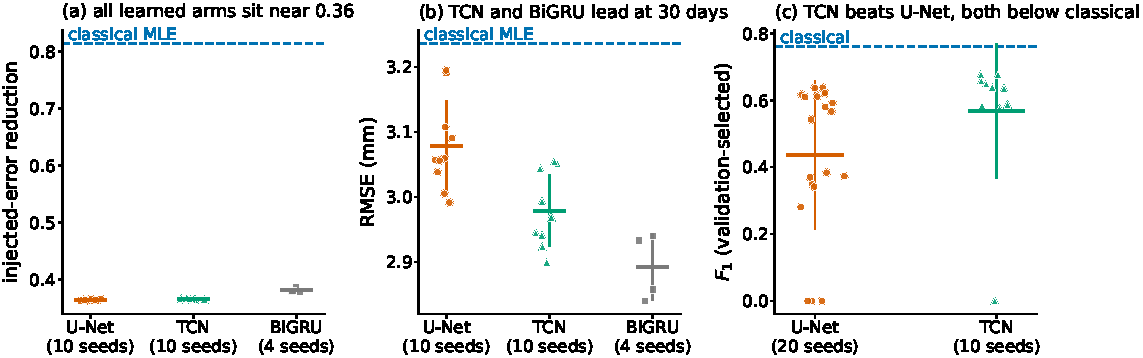
\includegraphics[width=\linewidth]{figures/fig10_architecture_seed.pdf}
\caption{Three architectures under one protocol. (a) Denoising error reduction
for the U-Net, TCN and BiGRU: the three means lie within $0.02$ of one another
and far below the trajectory MLE (dashed). (b) 30-day gap RMSE: TCN and BiGRU
are closer to the classical MLE than the U-Net, and all three beat linear
interpolation. (c) Detection at 8~mm: the TCN is ahead of the U-Net, and both
are below the classical detector (dashed). Dots are training seeds, horizontal
bars are means and vertical bars are $\pm$1~s.d.; the spread, not the mean
difference, dominates panel (c).}
\label{fig:architecture_seed}
\end{figure}


\section{Discussion}
\label{sec:discussion}

The three tasks do not support a single verdict, and the differences between
them are more informative than any average. The first version of this benchmark
reported a uniform classical win. Three of its ingredients do not survive the
revised protocol: the truth sat inside the parametric basis, the learned gap
filler was evaluated under a normalisation it was not trained with, and the
downstream noise model was re-estimated on denoised outputs. Correcting them
reverses the gap-filling verdict, makes the denoising verdict conditional, and
leaves detection negative.

\paragraph{The denoising advantage is a property of the truth family.}
On the in-family truth the trajectory model removes $0.790$ of the injected
error and the RTS smoother $0.791$, while the U-Net removes $0.366 \pm 0.002$
and the model-free decompositions lie between $0.232$ and $0.349$. That ordering
is expected: the truth is a trend plus constant harmonics with mild modulation,
which is almost exactly the basis of the parametric estimator. Moving the truth
outside that basis changes the ranking. The trajectory model falls to $-0.106$
and the RTS smoother to $-0.104$: on a signal it cannot represent, the fit adds
error rather than removing it. The model-free decompositions barely move, and
the U-Net, trained on the matching out-of-family generator, does not degrade at
all: it scores $0.363 \pm 0.001$. Scored with per-window normalisation, it is
above every model-free decomposition in both families. On the synthetic grid it
reaches $0.389 \pm 0.001$ in-family and $0.381 \pm 0.001$ out-of-family, against
$0.320$ and $0.318$ for the moving median and $0.317$ and $0.312$ for the
wavelet. The defensible statement is therefore narrower than a strong
learned-denoiser claim: the learned denoiser is the best non-parametric choice
in both families and the only learned arm that is nearly family-invariant, but
it remains far below the parametric estimator when the truth lies in its basis.
The earlier reading, in which the learned denoiser won only on the synthetic
grid and lost to the wavelet on real stations, was an artefact of whole-series
normalisation at inference.

\paragraph{Gap filling improves but does not win on the full real set.}
The first version evaluated the network with whole-series normalisation while
training it on per-window statistics. Scoring the same ten nets per window
removes the deficit: at 30 days the per-window U-Net reaches $3.07 \pm 0.03$~mm
on long synthetic records and $2.74 \pm 0.03$~mm on the 30-series real subset,
against $3.34$ and $2.93$ for linear interpolation and $3.79$ and $3.35$ for the
trajectory model. At 5 days it is $0.23$~mm behind SSA on synthetic records and
$0.05$~mm behind on real ones, and at 120 days the trajectory model remains
better ($3.99$ against $5.09 \pm 0.08$). The whole-series arm is not a
competitive configuration at any length. The correction does not extend to the
full held-out data: across all 201 test component series the U-Net ties linear
interpolation on NGL ($2.964$ against $2.967$~mm) and falls $0.06$~mm behind on
JPL ($3.293$ against $3.233$), and it leads by region only in Asia and Europe
(Sec.~\ref{sec:results:external}). The learned filler is therefore competitive
at intermediate gaps, and the first version's failure was an inference defect
rather than an architectural limit, but the corrected result is parity on real
data, not a product-level win. The defect is also a warning for the field: a
normalisation mismatch between training and inference can look like a
model-capacity failure, and a single-seed, single-protocol evaluation cannot
tell the two apart.

The mechanism behind the win is visible in the signal-error arm. The trajectory
model's error against the missing true signal stays near $0.7$~mm at every gap
length, because it extrapolates a low-order trend and harmonics; the
whole-series network reaches $5.97$~mm at 30 days and $61.0$~mm at 365 days.
The per-window network inherits the interpolation prior learned over gaps of
5--120 days, which is why it is competitive in the middle of that range and why
its advantage should not be extrapolated to year-long gaps, for which no
per-window measurement was made.

\paragraph{Detection: a better ranking does not give a better operating point.}
On synthetic offsets the classical detector has the higher validation-selected
$F_1$ at every amplitude, from $0.073$ against $0.0005$ at 2~mm to $0.975$
against $0.725$ at 25~mm. The learned field nevertheless has the higher average
precision at 16 and 25~mm ($0.648$ and $0.669$ against $0.208$ and $0.007$). The
two metrics answer different questions: average precision integrates over all
thresholds, while the deployed detector uses one threshold chosen on held-out
stations. The learned field orders large events well but transfers its operating
point poorly. On real catalogue labels the gap widens: classical $F_1$ is
$0.457 \pm 0.027$, the twenty U-Net seeds average $0.232 \pm 0.107$, the ten TCN
seeds $0.273 \pm 0.096$, and four seeds across the two architectures collapse to
essentially no detections. Where a learned seed does fire, its matched detections
sit closer to the catalogued epoch (absolute median delay $16.5$--$52.1$ days for
the U-Net and $7.8$--$39.9$ days for the TCN, against $69.7$ for the classical
detector), but it finds fewer events. The catalogue is not ground truth either: its dates may refer to
the earthquake rather than to the observable break, which is why the real-label
arm uses a 180-day tolerance. The comparison is nonetheless the one a geodesist
would make, and it does not show a learned advantage.

\paragraph{What the velocity product inherits.}
The corrected downstream test removes the earlier warning rather than changing
its mechanism. With the noise model estimated on the raw series and held fixed,
the trajectory MLE is unbiased ($-0.0024$~mm\,yr$^{-1}$) with a velocity RMSE of
$0.0586$~mm\,yr$^{-1}$, and the classical denoisers stay within
$0.0588$--$0.0616$. The U-Net denoiser reaches $0.0605$ (two seeds, $0.0600$ and
$0.0611$) with a bias of $-0.0034$, and the U-Net imputer is indistinguishable
from the classical fillers at $0.0586$. Calibration is $0.649$ for the
reference, $0.618$--$0.647$ for the classical denoisers and $0.628$ for the
learned denoiser, with 1$\sigma$ coverage of $0.389$, $0.444$--$0.472$ and
$0.458$ respectively. The values of the first version ($0.2087$ and $0.197$)
came from whole-series normalisation, which mismatches the statistics the
network was trained under; scoring window by window removes them, and the
learned arm is neither better nor worse than the classical denoisers by more
than $0.002$~mm\,yr$^{-1}$. Re-estimating the noise on a denoised output, the
other protocol of the first version, still collapses the reported uncertainty
for the trajectory and RTS outputs because they leave essentially no residual;
that arm is reported to explain the earlier number, not as a valid pipeline.
Adding a random-walk component lowers the reference RMSE from $0.0586$ to
$0.0690$ and the calibration ratio from $0.649$ to $0.575$; the U-Net denoiser
reaches $0.0698$ and the imputer $0.0690$, and the ordering is unchanged. The
product-level rule is therefore weaker than in the first version: no method,
learned or classical, improves a velocity that the joint trajectory/noise fit
already estimates, but learned denoising no longer damages the product. The
decision should be made on the product metric, not on the pointwise signal
error, because the two do not move together.

\paragraph{Architecture and seeds.}
The detection result is not a statement about one architecture or one draw. On
the real labels the seed standard deviation is $0.107$ for the U-Net and
$0.096$ for the TCN, nearly half the mean in both cases, and on synthetic
offsets at 8~mm the U-Net seed distribution has a standard deviation of $0.222$
around a mean of $0.436$. A TCN does better than the U-Net at every amplitude
above 4~mm ($0.829$ against $0.686$ at 16~mm, $0.791$ against $0.675$ at
25~mm), and the real-label ranking agrees ($0.273$ against $0.232$), but neither
reaches the classical operating point. Denoising is architecture-insensitive:
U-Net, TCN and BiGRU means are $0.364$, $0.365$ and $0.381$. Gap filling
separates them modestly, with the BiGRU best at 5 and 30 days ($2.378$ and
$2.892$~mm) and the TCN second ($2.401$ and $2.979$), but the BiGRU costs
$5.1$~h per seed against $6$~min for the TCN. The seed spread dominates the
architecture difference in detection; in gap filling the ordering is stable
across architectures, which is the stronger form of the result.

\paragraph{Limitations.}
The truth families are still constructed, not observed: the in-family and
out-of-family signals are deterministic functions with known parameters, and the
out-of-family generator is one choice among many. The real-label arm scores
against a catalogue, not against a measured break, and its 3$\sigma$ amplitude
filter removes weak continuity changes that a detector might still be expected
to find. All experiments are single-station; common-mode error and network
filtering are outside the protocol. The downstream arm uses six stations, two
components, three realisations and two U-Net seeds, so its calibration ratios
carry a wide interval and are read as a comparison across methods, not as an
absolute calibration of geodetic uncertainty; the untreated series itself covers
$0.389$ at 1$\sigma$ because of irregular sampling, and that shortfall is shared
by every method. The random-walk arm tests one amplitude ($1.0$~mm\,yr$^{-1/2}$)
and one noise model. The 365-day gap and the 16--25~mm offsets lie at or beyond
the training support and measure extrapolation rather than in-distribution
skill. The external centre arm is descriptive: it scores held-out JPL series
with networks trained on the same generators, not networks retrained at JPL,
so the design is a single primary analysis centre plus JPL, not a multi-centre
evaluation; its JPL group contains 18 component series against 183 for NGL. The
regional split is uneven, with 123 component series in Asia and six in the
residual group, so regional means outside Asia and North America rest on few
stations and are read as a consistency check on the ranking rather than as
regional predictions.


\section{Conclusions}
\label{sec:conclusion}

The question this benchmark asks is whether a learned method should replace a
well-implemented classical one in the GNSS coordinate-series pipeline. The
answer is task-specific, and the first version's uniform negative verdict does
not survive a protocol that removes three confounds: a truth inside the
parametric basis, a normalisation mismatch at inference, and a downstream noise
model re-estimated on denoised output.

Denoising is conditional on the truth family. The trajectory model and the RTS
smoother remove about four-fifths of the injected error when the truth is a
trend plus constant harmonics, but they add error when it is not. The learned
denoiser is nearly family-invariant, $0.366 \pm 0.002$ in-family and
$0.363 \pm 0.001$ out-of-family, and under per-window inference it beats every
model-free decomposition in both families; it stays well below the parametric
estimator when the truth lies in its basis. The earlier placement of the U-Net
below SSA and the wavelet came from whole-series normalisation at inference, not
from the network.

Gap filling is the task where a learned method gains the most under the
revised protocol, but the gain is confined to synthetic records; on real data
the learned filler is at parity at best. With per-window inference, which
matches the statistics used in
training, the U-Net is the best method at 30-day synthetic gaps ($3.07$ against
$3.34$~mm for linear interpolation). On the full held-out set of 201 component
series it reaches $2.964$~mm on NGL against $2.967$ for linear interpolation, a
tie, and $3.293$ on JPL against $3.233$, $0.06$~mm behind; by region it is
ahead only in Asia and Europe. It is slightly behind SSA at 5 days and behind
the trajectory model at 120 days. A TCN and the smaller BiGRU match or beat it
at 5 and 30 days, so the advantage is not specific to the encoder--decoder
design, though the BiGRU costs two orders of magnitude more to train. The
earlier failure was an inference defect, not an architectural limit; the
corrected result is a competitive learned method at intermediate gaps, not a
demonstrated improvement over interpolation on real data.

Offset detection remains a classical win at the operating point. The learned
field has higher average precision at large offsets, but its validation-selected
$F_1$ is lower at every amplitude, and on real catalogue labels it trails the
classical detector: $0.457 \pm 0.027$ for the classical arm, $0.232 \pm 0.107$
for the twenty U-Net seeds and $0.273 \pm 0.096$ for the ten TCN seeds, with
four of the thirty seeds collapsing. The TCN is ahead of the U-Net, so the
negative detection verdict does not depend on one architecture, but it is still
below the classical detector. The seed spread is part of the result, not noise
to be averaged away.

The velocity product narrows the case for learned pre-processing without
reversing it. Under protocol-matched inference no method improves the velocity:
the untreated series and classical denoisers sit at
$0.0586$--$0.0616$~mm\,yr$^{-1}$, the learned denoiser at $0.0605$ and the
learned imputer at $0.0586$. Calibration is likewise preserved
($0.618$--$0.649$ across methods). The earlier factor-of-$3.6$ degradation and
the calibration collapse to $0.197$ were produced by whole-series
normalisation, and they disappear when the network is scored window by window.
The random-walk arm lowers absolute accuracy for every method without changing
the ordering. The practical recommendation is therefore narrower than before:
neither learned nor classical denoising is a substitute for a joint
trajectory/noise fit upstream of a published velocity, and a learned gap filler
is a defensible alternative at 30-day synthetic gaps but has not shown an
advantage over linear interpolation on the full held-out real set. Learned
pre-processing carries no product-level penalty. The remaining product-level objection is that
it carries no gain either.

Two methodological lessons carry beyond this benchmark. A normalisation
mismatch between training and inference can mimic a capacity failure, so learned
pipelines must be scored under the protocol they were trained with before a
negative result is attributed to the model. And a downstream calibration
comparison is only as meaningful as the noise model attached to each method;
re-estimating that model on a denoised output is not a valid protocol, because
the denoiser has removed the information the estimator needs.

What remains open is a truth observed rather than constructed, a multi-station
treatment of common-mode error, and a learned detector trained and validated on
real catalogue labels with a pre-registered operating point. The benchmark and
its result files make those extensions measurable on the same frozen split.


\section*{Declarations}

\paragraph{Funding.}
The authors received no specific funding for this work.

\paragraph{Competing interests.}
The authors declare no competing interests.

\paragraph{Author contributions.}
Q.Z. designed the benchmark, implemented the methods and experiments, and
drafted the manuscript. Z.C. supervised the study and revised the manuscript.
Both authors approved the final version.

\paragraph{Data availability.}
The NGL daily series are publicly available from the Nevada Geodetic Laboratory
(\url{https://geodesy.unr.edu}) and the JPL series from the Jet Propulsion
Laboratory (\url{https://sideshow.jpl.nasa.gov/post/series.html}); the NGL
discontinuity catalogue is the public \texttt{steps.txt} file downloaded
2026-10-18 and identified in Sec.~\ref{sec:data}. The frozen station list, the
split file, the trained-network checkpoints and the result files that generate
every number in this paper are listed in the release manifest supplied with the
submission (file list and checksums); the archive itself will be deposited in a
public repository on acceptance, and no repository address is asserted here.

\paragraph{Code availability.}
The analysis code, training scripts, evaluation harness and figure scripts are
in the same release archive; their paths and checksums are given in the
manifest.

\clearpage
\bibliographystyle{spbasic}
\bibliography{refs}

\end{document}
